\chapter{Initial Prototypes}
\label{chap:initial-prototypes}

This chapter explores a failed approach to utilise Collaborative Filtering (CF) in attempting to solve this 
dissertation's research question. 
As part of the approach, popular datasets\footnote{\url{https://openpsychometrics.org/_rawdata/}} were utilised that others may use in solving similar problems to this dissertation.
A machine learning model classifier was trained on this dataset, and the results were unsatisfactory due to a lack of coverage by the questions in the dataset.

This chapter will describe the motivations behind the chosen approach, the implementation details, and then evaluate 
the results and describe why the experiment yielded unsatisfactory results. 

\section{Design Motivation}

In this section, we will describe the motivation behind this approach.
If we recall the research question as outlined in section \ref{sec:research-question},
we are seeking to design an RS that assists a user's exploration into college courses
by providing with them relevant, diverse, and serendipitous recommendations.
Among the three types of RSs described in section \ref{sec:common-rs-types},
Collaborative Filtering (CF) is more likely to provide serendipitous
recommendations, according to \cite{aggarwal2016recommender}.
This is because CF does not solely rely on what the user likes, rather it leverages the data of what other similar users also liked, 
increasing the likelihood of more surprising, but relevant recommendations, i.e. serendipity.
As also described in section \ref{sec:research-gap}, 
serendipity is the gold standard of RSs, and it would be incredibly useful in answering our research question by assisting the user in their exploration of college courses.
As a result, this chapter will explore a CF approach as it potentially provides more serendipitous recommendations.

It is worth mentioning that for the sake of brevity, 
this chapter will not feature a vivid description of the different strategies attempted to improve model performance.
Instead, we will focus on our best attempt in solving this problem through the CF approach.

\section{Datasets and Initial Challenges}

In section \ref{sec:research-gap}, we identified a research 
gap by leveraging a user's RIASEC model and academic interests to provide personalised college course recommendations.
However, in order to design a CF RS in this context, we need to find datasets with other users' college choice, and either their academic interests 
or RIASEC model.
To the best of our knowledge, this kind of data is not available in the Irish context.
As a result, we explored similar datasets outside of the Irish context.

A promising dataset in this context was published by OpenPsychometrics\footnote{\url{https://openpsychometrics.org/_rawdata/}} with data on over 140,000 individuals.
In this dataset, which will be referred to as the `RIASEC dataset', feature the results of a 48-question quiz which determined the user's RIASEC model.
This quiz asked the user how much they enjoyed certain activities on a 5-point Likert scale, i.e. 1 implied they dislike the activity, and a 5 implied they would enjoy the activity.
An example of a question is given in figure \ref{fig:op-quiz}.
As part of the quiz, the user was asked to provide their college major, which is crucial information in our context.
After some initial data cleaning, we were left with over 70,000 user's RIASEC quiz results and their college majors.
This kind of data would be essential in designing a CF RS.

\begin{figure}[H]
    \centering
    \fbox{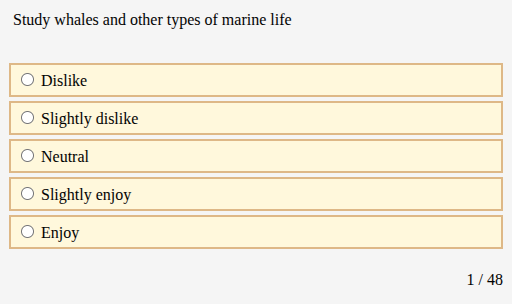
\includegraphics[scale=0.5]{images/op-question.png}}
    \caption{An example of a question given on the OpenPsychometrics RIASEC quiz.}
    \label{fig:op-quiz}
\end{figure}

However, as described in subsection \ref{sec:research-gap}, this dissertation seeks to design an RS that recommends specific Irish college courses,
as opposed to general areas of study.
The RIASEC dataset has been answered by users from all over the world, particularly from the USA.
As a result, there is a challenge in mapping the college majors that users provided in the RIASEC dataset, 
to specific Irish college courses.
Moreover, new Irish college courses are being created each year,
compounding the difficulty of this problem.

\section{Solution to Introduced Problems}

As a solution to the problem of specificity provided above, we can create more general categories of related college courses.
For example, we can 
group college majors/courses such as medicine, Nursing and Occupational Therapy under a ``healthcare" category.
The college majors in the RIASEC dataset can be placed into these categories,
and the college courses in the Irish college course dataset can also be placed into these categories.
Admittedly, a disadvantage of this solution is a loss of nuance that would occur in the mapping.
In other words, specific traits of particular college majors 
will get lost as they are combined into a more general category with other college majors.

We now need to find a dataset with college majors and associated college major categories.
A popular dataset on college majors in the USA\footnote{\url{https://github.com/fivethirtyeight/data/tree/master/college-majors}} 
was most appropriately applied to this problem. This dataset, which will be referred to as the `college major dataset', initially featured 174 college majors and categorised each college major 
under 15 categories.
However, in its initial form, this college major dataset failed to capture many of the college majors provided in the RIASEC dataset.
In addition to this, many of the college major categories were too broad, and were then split up into different college major categories.
As a result, this college major dataset underwent significant manual revisions, and the final form of this dataset is provided in table \ref{tab:college-major-dataset}.
After these significant manual revisions, the college major dataset featured over 200 college majors with 16 categories.

\newpage

\begin{table}[ht]
\centering
\tiny
\renewcommand{\arraystretch}{0.75} % <--- Reduces vertical padding between rows
\setlength{\tabcolsep}{3pt} % Tighten spacing to fit width
\begin{tabular}{ll p{0.5cm} ll p{0.5cm} ll}
\toprule
\textbf{Major} & \textbf{Category} && \textbf{Major} & \textbf{Category} && \textbf{Major} & \textbf{Category} \\
\midrule
acting & arts && english education & education && culinary arts & hospitality \\
animation & arts && health education & education && event management & hospitality \\
art and design & arts && history education & education && hospitality management & hospitality \\
commercial art & arts && language education & education && hotel management & hospitality \\
dance & arts && library science & education && tourism & hospitality \\
design & arts && mathematics education & education && tourism management & hospitality \\
drama & arts && music education & education && anthropology & humanities \\
fashion & arts && physical education & education && art history & humanities \\
fashion design & arts && psychology education & education && civilization studies & humanities \\
fashion merchandising & arts && science education & education && classical studies & humanities \\
film studies & arts && secondary education & education && comparative literature & humanities \\
fine arts & arts && social science education & education && english & humanities \\
graphic design & arts && special education & education && english literature & humanities \\
interior design & arts && aeronautical engineering & engineering && history & humanities \\
music & arts && aerospace engineering & engineering && intercultural studies & humanities \\
performing arts & arts && agricultural engineering & engineering && international studies & humanities \\
photography & arts && architectural engineering & engineering && liberal arts & humanities \\
product design & arts && architecture & engineering && literature & humanities \\
studio arts & arts && aviation studies & engineering && philosophy & humanities \\
theater & arts && biological engineering & engineering && religious studies & humanities \\
visual arts & arts && biomedical engineering & engineering && rhetoric & humanities \\
writing & arts && biotechnology & engineering && theology & humanities \\
child development & beh. health* && chemical engineering & engineering && criminal justice & law \\
clinical psychology & beh. health* && civil engineering & engineering && criminology & law \\
comm. disorders & beh. health* && computer engineering & engineering && government & law \\
counseling & beh. health* && construction studies & engineering && intl. relations & law \\
family science & beh. health* && electrical engineering & engineering && legal studies & law \\
human development & beh. health* && engineering mgmt. & engineering && paralegal studies & law \\
human services & beh. health* && engineering tech. & engineering && political science & law \\
mental health & beh. health* && environmental eng. & engineering && public admin. & law \\
occupational therapy & beh. health* && geological engineering & engineering && public policy & law \\
psychology & beh. health* && geophysical engineering & engineering && agricultural science & life science \\
rehabilitation & beh. health* && industrial engineering & engineering && biochemistry & life science \\
social work & beh. health* && industrial management & engineering && biology & life science \\
speech pathology & beh. health* && manufacturing eng. & engineering && biomedical science & life science \\
accounting & business && marine engineering & engineering && biopsychology & life science \\
accounting \& finance & business && materials engineering & engineering && botany & life science \\
actuarial science & business && materials science & engineering && cognitive science & life science \\
administration & business && mechanical engineering & engineering && ecology & life science \\
business admin. & business && metallurgical eng. & engineering && environmental science & life science \\
business mgmt. & business && mining engineering & engineering && food science & life science \\
e-commerce & business && nuclear engineering & engineering && genetics & life science \\
economics & business && petroleum engineering & engineering && health science & life science \\
entrepreneurship & business && chinese & foreign languages && horticulture & life science \\
finance & business && english language & foreign languages && marine biology & life science \\
human resources & business && french & foreign languages && microbiology & life science \\
HR management & business && german & foreign languages && molecular biology & life science \\
intl. business & business && greek & foreign languages && neuroscience & life science \\
logistics & business && italian & foreign languages && pharmacology & life science \\
management & business && japanese & foreign languages && physiology & life science \\
mgmt. info. systems & business && korean & foreign languages && zoology & life science \\
marketing & business && latin & foreign languages && astronomy & physical science \\
operations mgmt. & business && linguistics & foreign languages && astrophysics & physical science \\
advertising & comms. && portuguese & foreign languages && atmospheric science & phys. science \\
journalism & comms. && russian & foreign languages && chemistry & physical science \\
mass media & comms. && spanish & foreign languages && earth science & physical science \\
public relations & comms. && translation & foreign languages && forensic science & phys. science \\
computer info. sys. & comp. \& math && community health & healthcare && geology & physical science \\
computer networking & comp. \& math && dental hygiene & healthcare && geoscience & physical science \\
computer science & comp. \& math && dental technology & healthcare && industrial tech. & phys. science \\
computer systems & comp. \& math && dentistry & healthcare && meteorology & physical science \\
cyber security & comp. \& math && health admin. & healthcare && physics & physical science \\
information science & comp. \& math && health services & healthcare && radiology & physical science \\
information systems & comp. \& math && medic & healthcare && behavioral science & social science \\
info. technology & comp. \& math && medical admin. & healthcare && geography & social science \\
mathematics & comp. \& math && medical assisting & healthcare && sociology & social science \\
programming & comp. \& math && medicine & healthcare && athletic training & sport \\
software eng. & comp. \& math && medicine technology & healthcare && exercise \& sport & sport \\
statistics & comp. \& math && midwifery & healthcare && exercise physiology & sport \\
telecommunications & comp. \& math && nursing & healthcare && exercise science & sport \\
adult education & education && nutrition science & healthcare && kinesiology & sport \\
art education & education && pharmacy & healthcare && physical therapy & sport \\
early childhood & education && public health & healthcare && sports management & sport \\
educational admin. & education && veterinarian & healthcare && sports medicine & sport \\
elementary education & education && vet. technology & healthcare &&  &  \\
\bottomrule
\multicolumn{8}{l}{\textit{*beh. health = behavioural health and human services}} \\
\end{tabular}
\caption{Complete list of College Majors and Categories.}
\label{tab:college-major-dataset}
\end{table}

We now have a college major dataset with over 200 college majors and 16 associated college major categories, 
and a RIASEC dataset with over 70,000 user's college majors and the results of their RIASEC quiz.
Using a pre-processing script as given in section \ref{sec:preprocessing-script},
we can categorise each of the $\sim$70,000 users in the RIASEC dataset into one of 16 college major categories as provided in the college major dataset.
This augmented dataset will be instrumental in training a Machine Learning model to predict a user's college major category from the results
of this RIASEC quiz, which will be explored in the next section.

\section{Machine Learning Model Selection}

From the work in the last section, we now have a dataset with over 70,000 user's RIASEC quiz results, and their college major category.
This can be reconceptualised in the context of a Machine Learning (ML) problem: 
we have 48 input features, and one output variable.
In this case, each input feature is a rating from 1--5, indicating the user's enjoyment towards a particular task,
and the output is one of 16 college major categories.

Many different ML models were trained on this data, and they were tested on unseen data to gather evaluation metrics,
in particular: top-1 and top-3 accuracy.
The ML model with the best
top-1 and top-3 accuracy was the Histogram-based Gradient Boosting Classifier (HGBC), with its implementation details given in listing \ref{lst:hgbm-implementation} below:

\begin{lstlisting}[caption={Histogram Gradient Boosting Classifier Implementation}, label={lst:hgbm-implementation}]
hist_gradient_boosting_machines_model = HistGradientBoostingClassifier(
        class_weight='balanced',
        l2_regularization=1.0
    )
\end{lstlisting}

This implementation of a HGBC achieved a top-1 accuracy of 0.319, and a top-3 accuracy of 0.606.
In other words for the unseen test set, this HGBC implementation predicted the user's college major category correctly in 31.9\% of cases (top-1 accuracy), 
and in 60.6\% of cases, the model predicted the user's college major category correctly in its first 3 predictions (top-3 accuracy).
Seeing as this implementation of the HGBC model had the best performance metrics, we can evaluate its performance further in the next section.

\section{Model Evaluation}

In this section we will take a closer look in evaluating the chosen HGBC model's performance.
In figure \ref{fig:confusion-matrix} below, we can observe the Confusion Matrix of the chosen model, 
showcasing the recall scores.

\begin{figure}[H]
    \centering
    \fbox{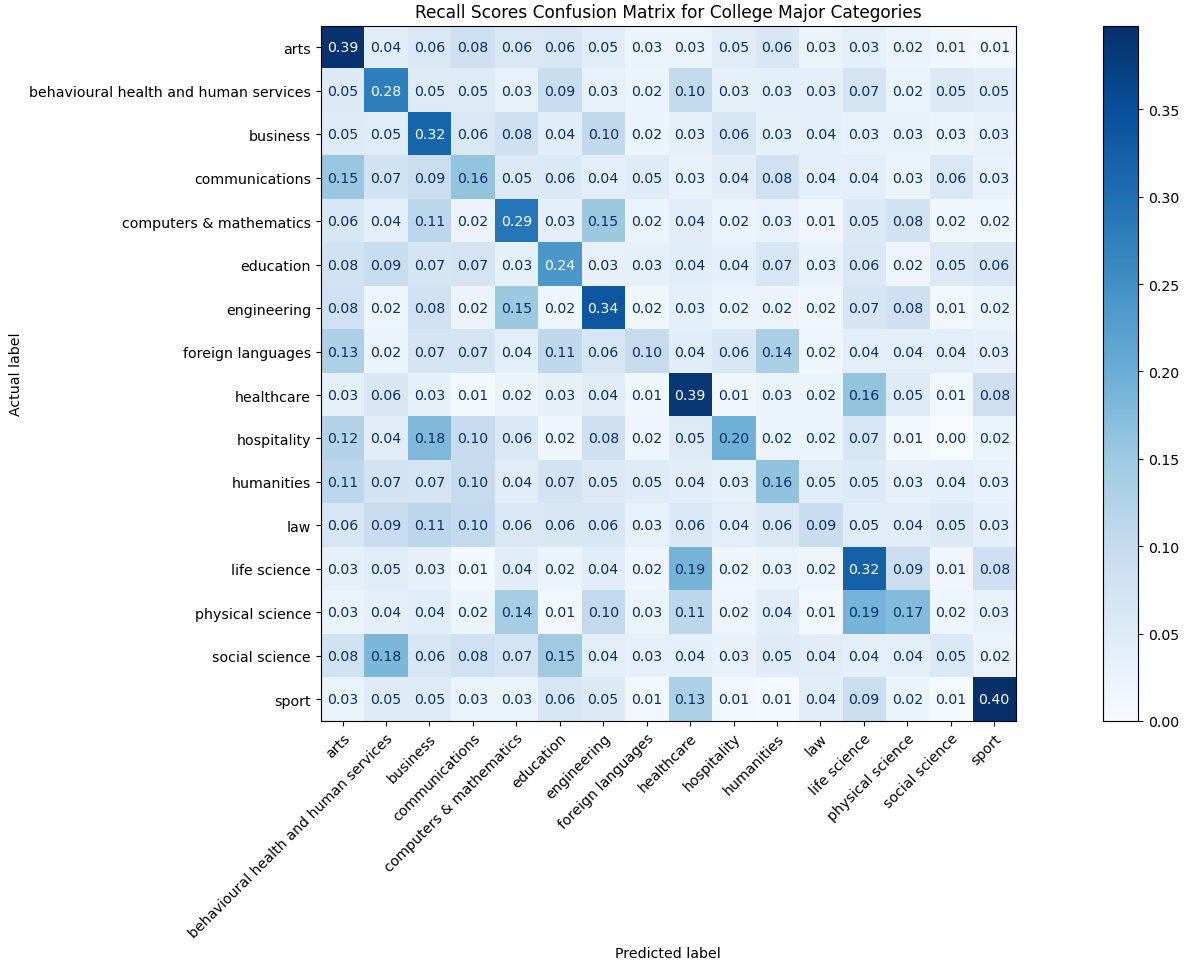
\includegraphics[scale=0.35]{images/recall-confusion-matrix-better.png}}
    \caption{A Confusion Matrix for Recall scores on the HGBC model.}
    \label{fig:confusion-matrix}
\end{figure}

To take one example, we can observe that the model achieved a recall score of 0.4 for the ``sports" college major category,
meaning that of all the users with ``sports'' as their college major category, 
the model correctly predicted ``sports'' for these users 40\% of the time.
Relatively speaking, we can see that this recall score of 0.4 is the highest performing recall score
out of all the other college major categories.
In particular, we can see the model struggling with some college major categories, such as ``foreign languages'' with 
a recall score of 0.1, and ``social science'' with a score of 0.05,
meaning that the model correctly predicts the user's college major category 10\% and 5\% of the time respectively.

Evidently speaking, the performance of this model was disappointing as demonstrated through the low recall scores referenced above.
Many different ML models with differing configurations were applied to the problem, failing to provide any improvements to this HGBC implementation.
As well as this, the college major dataset underwent significant manual revisions - adding new college majors and splitting up different college major 
categories, all failed attempts to improve the model's performance.

\section{Limitations of the Approach}

In the previous section, we established the poor performance of this model in predicting the user's college major category given the results of a 48-question RIASEC quiz.
In this section, we will provide more insights as to why the model with these popular datasets performed poorly.

In the context of predicting a user's college major, the primary limitation of the chosen RIASEC dataset is the lack of coverage by the questions.
In other words, the 48 questions do not adequately cover many areas of study,
which we believe is the primary reason behind the poor performance behind the model.
For example, if we revisit figure \ref{fig:confusion-matrix}, we can observe very poor model performance on the ``foreign languages'' category, with a recall score of 0.1.
This is simply because there are no questions in the RIASEC dataset that are explicitly related to languages or linguistics.
To provide another example, we can observe very poor recall scores for the ``law'' category, most likely because
there are no questions in the quiz that are explicitly related to law or government.
Without this data, the model finds it very difficult to discern if a user is studying in the ``foreign languages" or ``law'' categories, explaining the model's poor performance on these categories.

Due to this limitation, we found this dataset and subsequent approach to be inadequate in solving our problem, due to the poor recall scores as reported in figure \ref{fig:confusion-matrix}.
In spite of many efforts to improve the model's performance through significant manual revisions to the college major dataset,
and testing multiple different ML models and configurations,
the performance of the model was still deemed unsatisfactory.

\section{Chapter Summary}

In this chapter, we explored an approach to solving this dissertation's research question by 
utilising a very popular RIASEC dataset.
There was a description of the motivation in using this dataset, followed by an explanation of the various data engineering 
performed on both datasets in order to make it more suitable for a traditional ML problem.
We evaluated the performance of the best performing model, and found the results to be unsatisfactory.
Ultimately, we believe the unsatisfactory results to be a result of the poor coverage of the 48 questions on many different fields of study.
As a result, we believe that a dataset such as this may not be particularly useful in solving a problem similar to the one addressed in this dissertation.
That being said, we felt it was worth writing about our inadequate solutions in this chapter, 
firstly because of the popularity of this dataset,
and secondly to add a useful contribution to the literature.

\chapter{}

\section{Preprocessing script for college course/major classification}
\label{sec:preprocessing-script}

The following Python script was used to preprocess the names of college course titles and college majors.

\begin{lstlisting}
stemmer = SnowballStemmer("english")

def preprocess_college_title(text):
    text = text.lower()
    text = re.sub(r'[\.\?=!#\'`\*]', '', text) # remove certain symbols
    text = re.sub(r'\d+', '', text) # remove numbers

    for abbreviation, expanded_college_major in ABBREVIATIONS_MAP.items():
        
        pattern = r'\b' + re.escape(abbreviation) + r'\b'
        text = re.sub(pattern, expanded_college_major, text)

    # substitute certain symbols for spaces
    text = re.sub(r'[\(\)\{\}\[\]&/+,;:\\|\-]', ' ', text)

    text = text.strip()

    tokens = word_tokenize(text)
    cleaned_tokens = []
    for word in tokens:
        if word not in stop_words:
            stemmed_word = stemmer.stem(word)

            if stemmed_word not in cleaned_tokens:
                cleaned_tokens.append(stemmed_word)

            if len(cleaned_tokens) > 1 and "scienc" in cleaned_tokens:
                cleaned_tokens.remove("scienc")

    cleaned_tokens.sort()
    return ' '.join(cleaned_tokens)

ABBREVIATIONS_MAP = {
    'maths': 'mathematics',
    'teacher': 'teaching',
    'teaching': 'education',
    'pharmaceutical': 'pharmacy',
    'technician': 'technology',
    'admin': 'administration',
    'bio': 'biological',
    'phy': 'physics',
    'chem': 'chemistry',
    'chemistry': 'chemical',
    'dentist': 'dentistry',
    'dental': 'dentistry',
    'agri': 'agriculture',
    'ag': 'agriculture',
    'hrm': 'human resource management',
    'it': 'information technology',
    'ict': 'information and communication technology',
    'tech': 'technology',
    'llb': 'law',
    'bcl': 'civil law',
    'mgt': 'management',
    'gaeilge': 'irish'
}

\end{lstlisting}

\section{RIASEC Trait distribution per Academic Interest}
\label{sec:riasec-trait-dist}

\begin{figure}[H]
    \centering
    \begin{subfigure}[b]{0.48\linewidth}
        \centering
        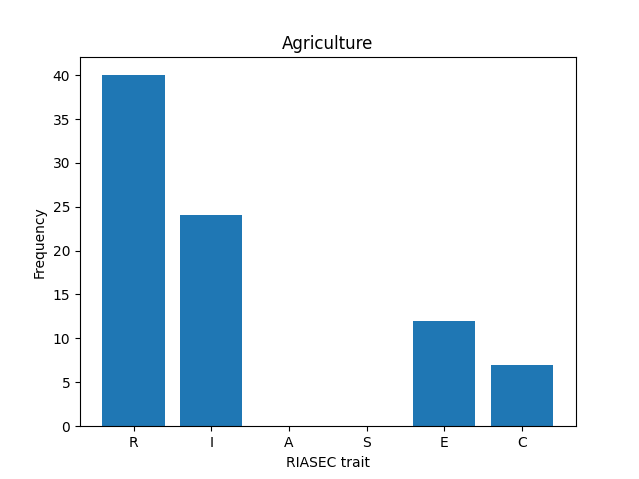
\includegraphics[width=\linewidth]{images/agriculture-distribution.png}
        \caption{Agriculture}
    \end{subfigure}
    \hfill
    \begin{subfigure}[b]{0.48\linewidth}
        \centering
        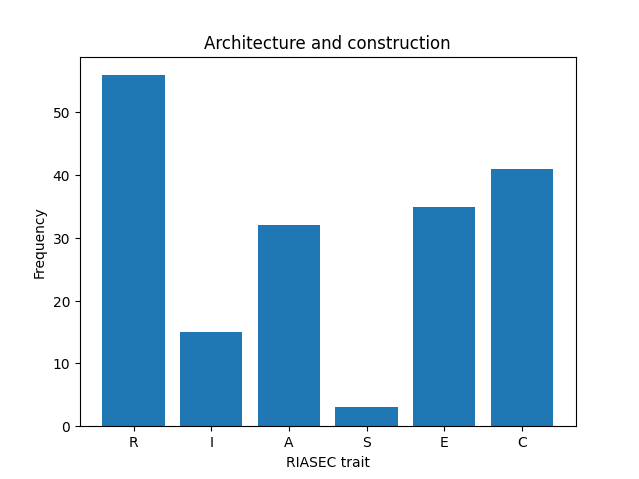
\includegraphics[width=\linewidth]{images/architecture-distribution.png}
        \caption{Architecture \& Construction}
    \end{subfigure}
    \begin{subfigure}[b]{0.48\linewidth}
        \centering
        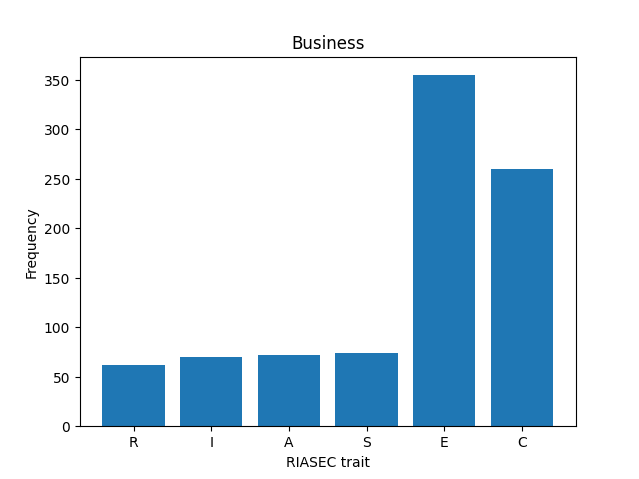
\includegraphics[width=\linewidth]{images/business-distribution.png}
        \caption{Business}
    \end{subfigure}
    \hfill
    \begin{subfigure}[b]{0.48\linewidth}
        \centering
        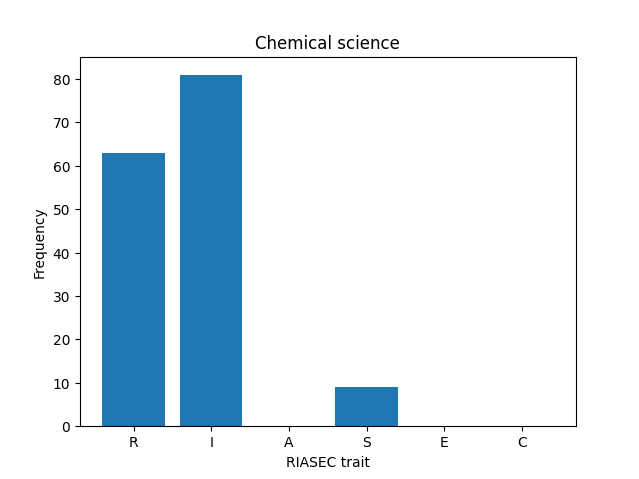
\includegraphics[width=\linewidth]{images/chem-distribution.png}
        \caption{Chemical Science}
    \end{subfigure}
    \begin{subfigure}[b]{0.48\linewidth}
        \centering
        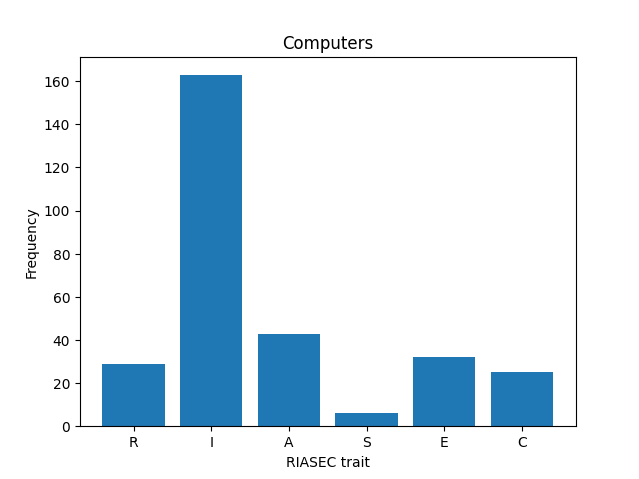
\includegraphics[width=\linewidth]{images/comp-distribution.png}
        \caption{Computers}
    \end{subfigure}
    \hfill
    \begin{subfigure}[b]{0.48\linewidth}
        \centering
        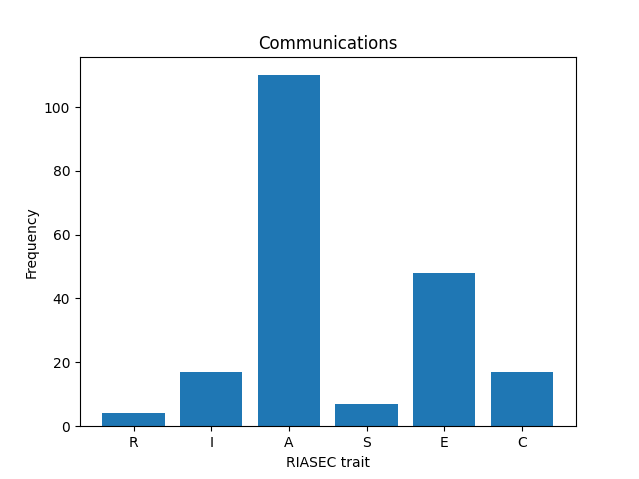
\includegraphics[width=\linewidth]{images/comms-distribution.png}
        \caption{Communications}
    \end{subfigure}
    \caption{RIASEC trait distribution across academic interests.}
\end{figure}

\begin{figure}[H]
    \centering
    \begin{subfigure}[b]{0.48\linewidth}
        \centering
        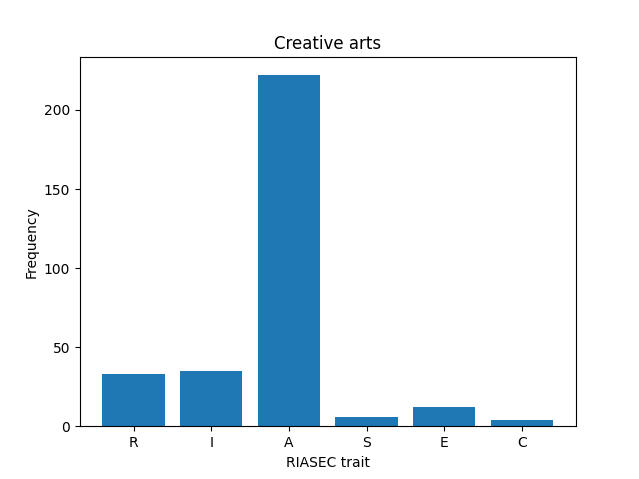
\includegraphics[width=\linewidth]{images/arts-distribution.png}
        \caption{Creative Arts}
    \end{subfigure}
    \hfill
    \begin{subfigure}[b]{0.48\linewidth}
        \centering
        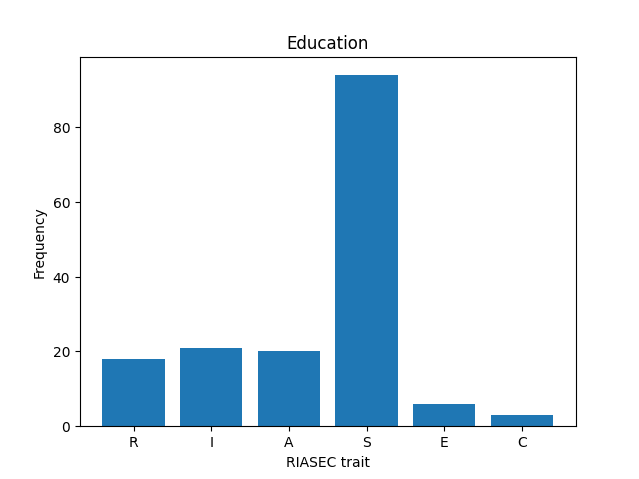
\includegraphics[width=\linewidth]{images/educ-distribution.png}
        \caption{Education}
    \end{subfigure}
    \begin{subfigure}[b]{0.48\linewidth}
        \centering
        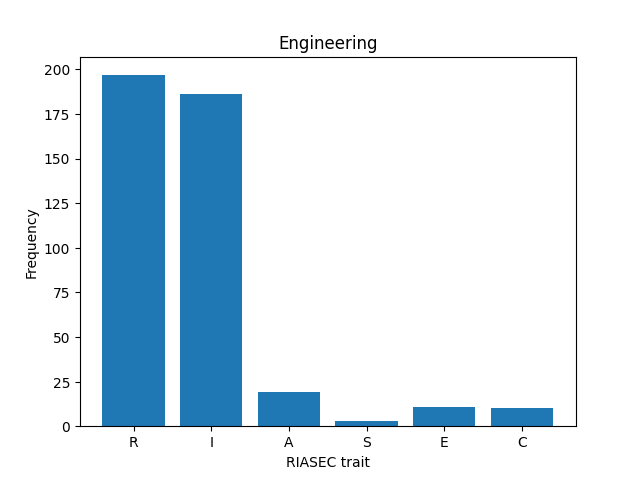
\includegraphics[width=\linewidth]{images/eng-distribution.png}
        \caption{Engineering}
    \end{subfigure}
    \hfill
    \begin{subfigure}[b]{0.48\linewidth}
        \centering
        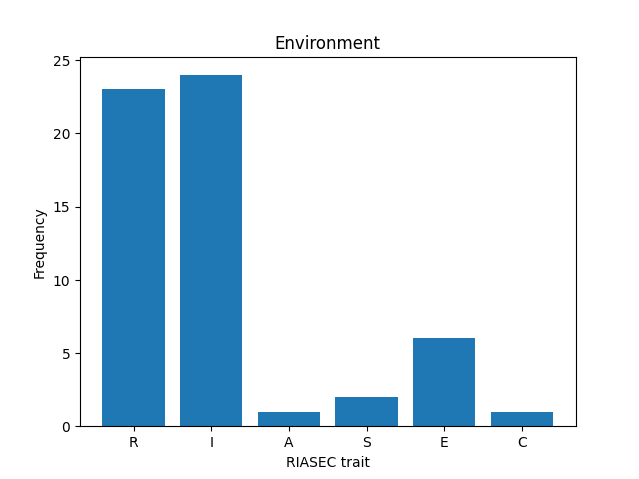
\includegraphics[width=\linewidth]{images/env--distribution.png}
        \caption{Environment}
    \end{subfigure}
    \begin{subfigure}[b]{0.48\linewidth}
        \centering
        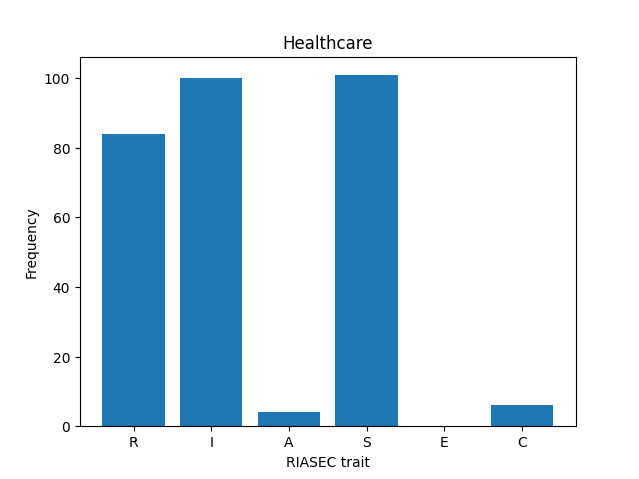
\includegraphics[width=\linewidth]{images/health-distribution.png}
        \caption{Healthcare}
    \end{subfigure}
    \hfill
    \begin{subfigure}[b]{0.48\linewidth}
        \centering
        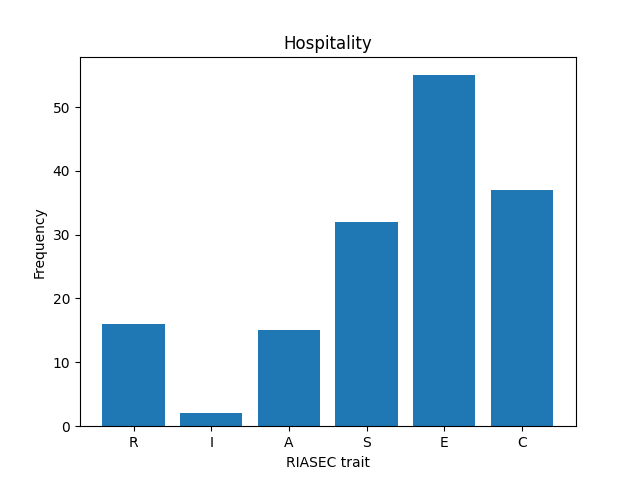
\includegraphics[width=\linewidth]{images/hosp-distribution.png}
        \caption{Hospitality}
    \end{subfigure}
    \caption{RIASEC trait distribution across academic interests.}
\end{figure}

\begin{figure}[H]
    \centering
    \begin{subfigure}[b]{0.48\linewidth}
        \centering
        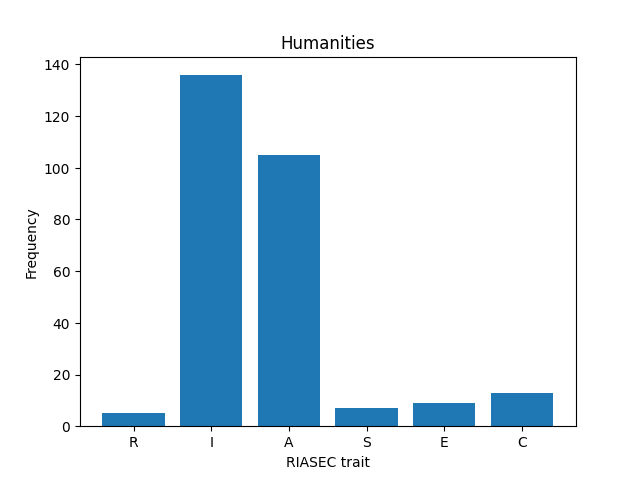
\includegraphics[width=\linewidth]{images/human--distribution.png}
        \caption{Humanities}
    \end{subfigure}
    \hfill
    \begin{subfigure}[b]{0.48\linewidth}
        \centering
        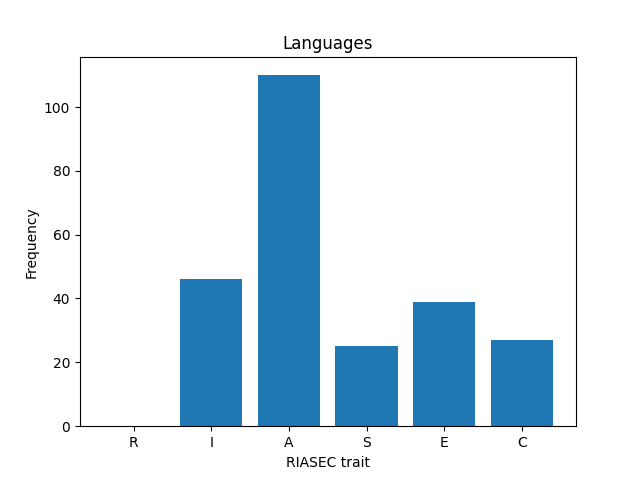
\includegraphics[width=\linewidth]{images/lang-distribution.png}
        \caption{Languages}
    \end{subfigure}
    \begin{subfigure}[b]{0.48\linewidth}
        \centering
        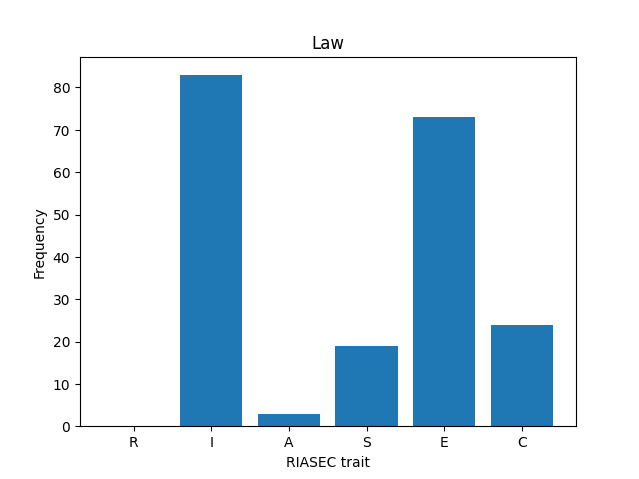
\includegraphics[width=\linewidth]{images/law-distribution.png}
        \caption{Law}
    \end{subfigure}
    \begin{subfigure}[b]{0.48\linewidth}
        \centering
        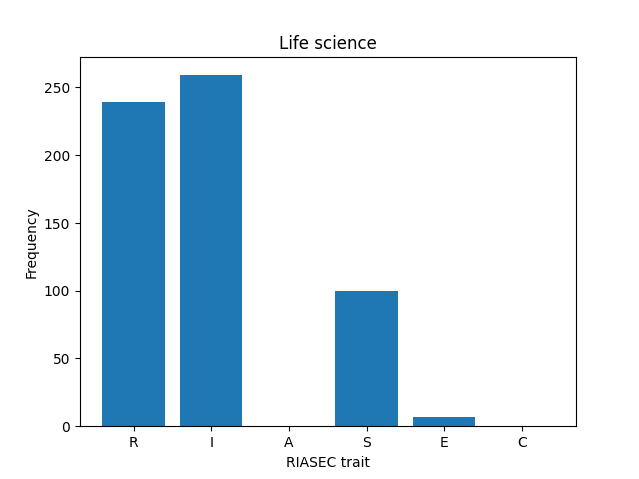
\includegraphics[width=\linewidth]{images/life-distribution.png}
        \caption{Life Science}
    \end{subfigure}
    \hfill
    \begin{subfigure}[b]{0.48\linewidth}
        \centering
        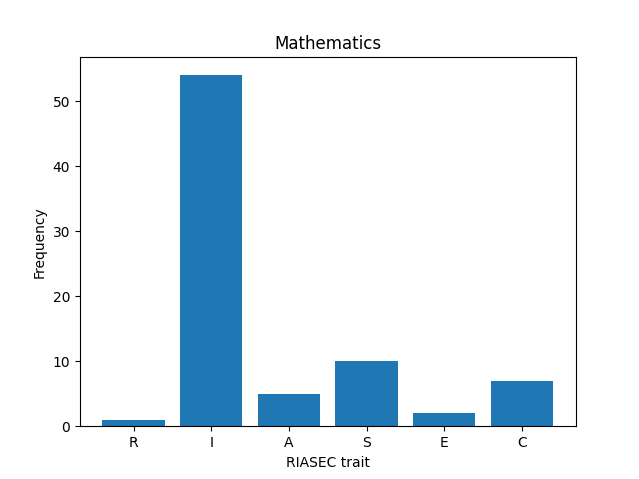
\includegraphics[width=\linewidth]{images/math-distribution.png}
        \caption{Mathematics}
    \end{subfigure}
    \begin{subfigure}[b]{0.48\linewidth}
        \centering
        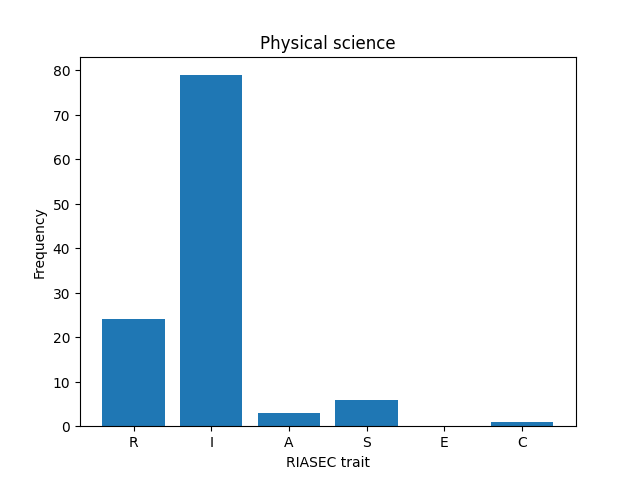
\includegraphics[width=\linewidth]{images/phy-distribution.png}
        \caption{Physical Science}
    \end{subfigure}
    \caption{RIASEC trait distribution across academic interests.}
\end{figure}

\begin{figure}[H]
    \centering
    \begin{subfigure}[b]{0.48\linewidth}
        \centering
        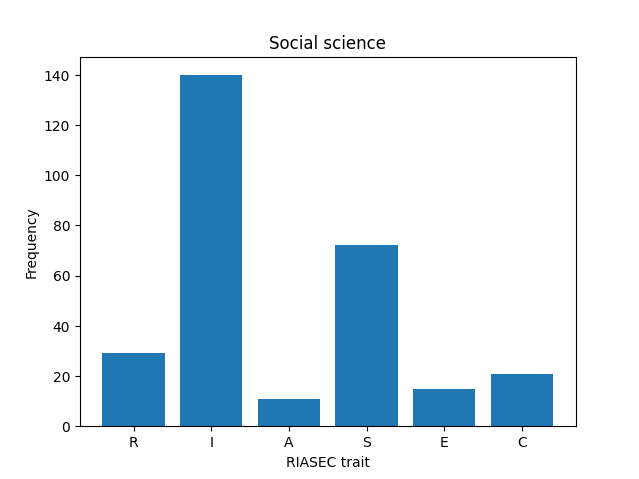
\includegraphics[width=\linewidth]{images/social-distribution.png}
        \caption{Social Science}
    \end{subfigure}
    \hfill
    \begin{subfigure}[b]{0.48\linewidth}
        \centering
        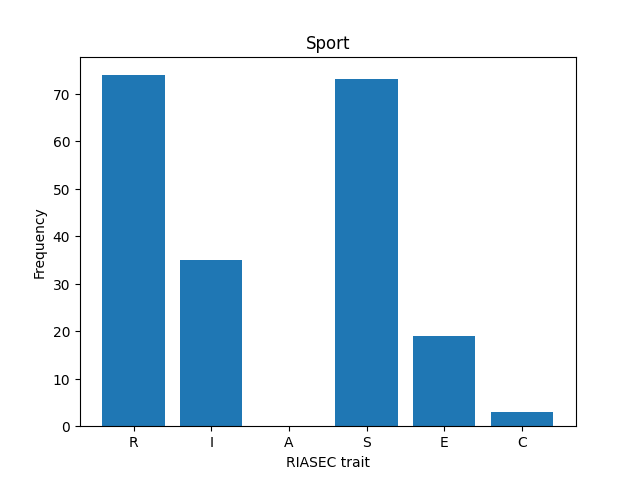
\includegraphics[width=\linewidth]{images/sport-distribution.png}
        \caption{Sport}
    \end{subfigure}
    \begin{subfigure}[b]{0.48\linewidth}
        \centering
        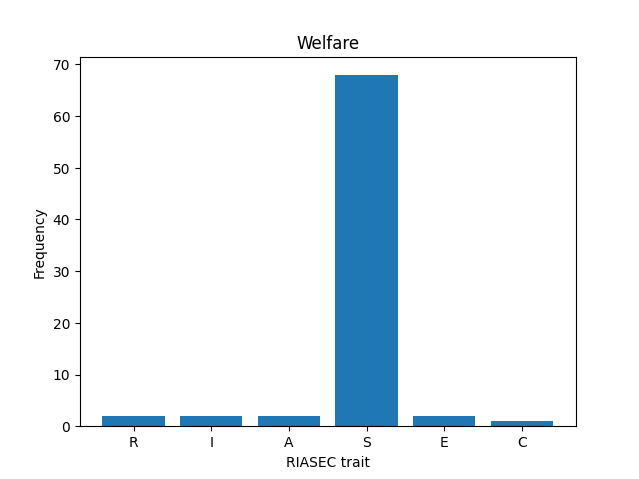
\includegraphics[width=\linewidth]{images/welfare-distribution.png}
        \caption{Welfare}
    \end{subfigure}
    \caption{RIASEC trait distribution across academic interests.}
\end{figure}

\section{All 126 Academic Interest Questions}
\label{sec:all-126-questions}

\begin{table}[H]
\centering
\begin{tabular}{|c|c|}
\hline
\multicolumn{2}{|c|}{\textbf{Agriculture}}\\
\hline
\hline
\textbf{Activity} & \textbf{RIASEC Trait}\\
\hline
Handle and care for livestock on a farm & \multirow{2}{*}{realistic}\\
\cline{1-1}
Repair and maintain high-tech farm machinery & \\
\hline
Research plant genetics for better crop yields & \multirow{2}{*}{investigative}\\
\cline{1-1}
Analyse soil chemistry to improve land health & \\
\hline
Sell agricultural products at a market to farmers & enterprising\\
\hline
Organise and track the financial accounts of a farm & conventional\\
\hline
\end{tabular}
\end{table}

\begin{table}[H]
\centering
\begin{tabular}{|c|c|}
\hline
\multicolumn{2}{|c|}{\textbf{Architecture \& Construction}}\\
\hline
\hline
\textbf{Activity} & \textbf{RIASEC Trait}\\
\hline
Draft technical drawings of building joints & \multirow{2}{*}{realistic}\\
\cline{1-1}
Build scale models to test structural strength & \\
\hline
Analyse how new building materials affect temperature & investigative\\
\hline
Design the aesthetic look of a new building & artistic\\
\hline
Lead site meetings to keep projects on track & enterprising\\
\hline
Check that building plans follow all safety laws & conventional\\
\hline
\end{tabular}
\end{table}

\begin{table}[H]
\centering
\begin{tabular}{|c|c|}
\hline
\multicolumn{2}{|c|}{\textbf{Business}}\\
\hline
\hline
\textbf{Activity} & \textbf{RIASEC Trait}\\
\hline
Negotiate with suppliers to lower business costs & \multirow{3}{*}{enterprising}\\
\cline{1-1}
Manage a sales team to exceed revenue targets & \\
\cline{1-1}
Pitch innovative business ideas to investors & \\
\hline
Organise company budgets and financial reports & \multirow{3}{*}{conventional}\\
\cline{1-1}
Maintain accurate business records and data & \\
\cline{1-1}
Coordinate complex logistics and supply chains & \\
\hline
\end{tabular}
\end{table}

\begin{table}[H]
\centering
\begin{tabular}{|c|c|}
\hline
\multicolumn{2}{|c|}{\textbf{Chemical Science}}\\
\hline
\hline
\textbf{Activity} & \textbf{RIASEC Trait}\\
\hline
Research how proteins change to fight specific diseases & \multirow{4}{*}{investigative}\\
\cline{1-1}
Discover how new drugs interact with human cells & \\
\cline{1-1}
Research how catalysts speed up chemical reactions & \\
\cline{1-1}
Analyse unknown substances to find their chemical makeup & \\
\hline
Mix raw ingredients to create skincare products & \multirow{2}{*}{realistic}\\
\cline{1-1}
Mix chemical compounds to create new products & \\
\hline
\end{tabular}
\end{table}

\begin{table}[H]
\centering
\begin{tabular}{|c|c|}
\hline
\multicolumn{2}{|c|}{\textbf{Computers}}\\
\hline
\hline
\textbf{Activity} & \textbf{RIASEC Trait}\\
\hline
Assemble and configure high-performance servers & realistic\\
\hline
Design a software application to handle millions of users & investigative\\
\hline
Fix hardware problems found in error logs & realistic\\
\hline
Organise and manage large databases of information & conventional\\
\hline
Optimise a computer program to run more efficiently & \multirow{2}{*}{investigative}\\
\cline{1-1}
Develop the code for a search engine & \\
\hline
\end{tabular}
\end{table}

\begin{table}[H]
\centering
\begin{tabular}{|c|c|}
\hline
\multicolumn{2}{|c|}{\textbf{Communications}}\\
\hline
\hline
\textbf{Activity} & \textbf{RIASEC Trait}\\
\hline
Build a viral social media campaign for a brand & \multirow{2}{*}{enterprising}\\
\cline{1-1}
Pitch a creative vision to launch a new product & \\
\hline
Design the logo and visual identity for a music festival & \multirow{3}{*}{artistic}\\
\cline{1-1}
Write an opinion piece for a respected newspaper & \\
\cline{1-1}
Direct a short film for a company's marketing campaign & \\
\hline
Investigate a news article to ensure 100\% truth & investigative\\
\hline
\end{tabular}
\end{table}

\begin{table}[H]
\centering
\begin{tabular}{|c|c|}
\hline
\multicolumn{2}{|c|}{\textbf{Creative Arts}}\\
\hline
\hline
\textbf{Activity} & \textbf{RIASEC Trait}\\
\hline
Create original paintings or drawings for exhibition & \multirow{5}{*}{artistic}\\
\cline{1-1}
Choreograph and perform expressive dance routines & \\
\cline{1-1}
Compose and perform an original piece of music & \\
\cline{1-1}
Perform lead roles in professional theatre or film & \\
\cline{1-1}
Write original stories or poetry & \\
\hline
Hand-craft original ceramic or pottery artworks & realistic\\
\hline
\end{tabular}
\end{table}

\begin{table}[H]
\centering
\begin{tabular}{|c|c|}
\hline
\multicolumn{2}{|c|}{\textbf{Education}}\\
\hline
\hline
\textbf{Activity} & \textbf{RIASEC Trait}\\
\hline
Create original lesson plans and activities for a class & artistic\\
\hline
Teach new concepts to a class of students & \multirow{5}{*}{social}\\
\cline{1-1}
Tutor students who need specialised support & \\
\cline{1-1}
Manage classroom behavior and group dynamics & \\
\cline{1-1}
Mentor young people to reach their potential & \\
\cline{1-1}
Explain complex theories in very simple ways & \\
\hline
\end{tabular}
\end{table}

\begin{table}[H]
\centering
\begin{tabular}{|c|c|}
\hline
\multicolumn{2}{|c|}{\textbf{Engineering}}\\
\hline
\hline
\textbf{Activity} & \textbf{RIASEC Trait}\\
\hline
Analyse thermal data to improve engine efficiency & \multirow{3}{*}{investigative}\\
\cline{1-1}
Analyse brain signals to control robotic limbs & \\
\cline{1-1}
Analyse airflow patterns to reduce aircraft drag & \\
\hline
Build a mini airplane with electrical motors & \multirow{3}{*}{realistic}\\
\cline{1-1}
Fix technical faults in industrial machinery & \\
\cline{1-1}
Build and calibrate electronic medical devices & \\
\hline
\end{tabular}
\end{table}

\begin{table}[H]
\centering
\begin{tabular}{|c|c|}
\hline
\multicolumn{2}{|c|}{\textbf{Environment}}\\
\hline
\hline
\textbf{Activity} & \textbf{RIASEC Trait}\\
\hline
Restore natural habitats by planting trees & \multirow{2}{*}{realistic}\\
\cline{1-1}
Build solar-powered water filtration systems & \\
\hline
Research new laws to reward companies for lowering carbon & \multirow{2}{*}{investigative}\\
\cline{1-1}
Analyse water samples to track the spread of microplastics & \\
\hline
Encourage firms to use sustainable packaging & \multirow{2}{*}{enterprising}\\
\cline{1-1}
Lead a campaign to convince a city to go carbon neutral & \\
\hline
\end{tabular}
\end{table}

\begin{table}[H]
\centering
\begin{tabular}{|c|c|}
\hline
\multicolumn{2}{|c|}{\textbf{Healthcare}}\\
\hline
\hline
\textbf{Activity} & \textbf{RIASEC Trait}\\
\hline
Evaluate a patient's symptoms to diagnose illnesses & \multirow{2}{*}{investigative}\\
\cline{1-1}
Research the biological mechanisms of the human body & \\
\hline
Provide direct care to sick patients & \multirow{2}{*}{social}\\
\cline{1-1}
Assist patients with physical rehabilitation & \\
\hline
Perform clinical procedures or surgeries & \multirow{2}{*}{realistic}\\
\cline{1-1}
Administer emergency first aid treatments & \\
\hline
\end{tabular}
\end{table}

\begin{table}[H]
\centering
\begin{tabular}{|c|c|}
\hline
\multicolumn{2}{|c|}{\textbf{Hospitality}}\\
\hline
\hline
\textbf{Activity} & \textbf{RIASEC Trait}\\
\hline
Manage and coordinate large-scale events & \multirow{2}{*}{enterprising}\\
\cline{1-1}
Lead the daily operations of a hotel & \\
\hline
Serve and help guests in a luxury setting & social\\
\hline
Cook and prepare food in a professional kitchen & realistic\\
\hline
Organise detailed travel plans for clients & conventional\\
\hline
Direct and lead staff in a busy restaurant & enterprising\\
\hline
\end{tabular}
\end{table}

\begin{table}[H]
\centering
\begin{tabular}{|c|c|}
\hline
\multicolumn{2}{|c|}{\textbf{Humanities}}\\
\hline
\hline
\textbf{Activity} & \textbf{RIASEC Trait}\\
\hline
Write creative essays on culture or history & \multirow{3}{*}{artistic}\\
\cline{1-1}
Design museum exhibits to tell history stories & \\
\cline{1-1}
Critique and review modern works of art & \\
\hline
Investigate different philosophical ideas & \multirow{3}{*}{investigative}\\
\cline{1-1}
Analyse themes in classic literature and art & \\
\cline{1-1}
Research how ancient civilisations lived & \\
\hline
\end{tabular}
\end{table}

\begin{table}[H]
\centering
\begin{tabular}{|c|c|}
\hline
\multicolumn{2}{|c|}{\textbf{Languages}}\\
\hline
\hline
\textbf{Activity} & \textbf{RIASEC Trait}\\
\hline
Analyse the grammatical structure of languages & investigative\\
\hline
Speak fluently in a foreign language & \multirow{3}{*}{social}\\
\cline{1-1}
Translate for people in professional settings &\\
\cline{1-1}
Teach a language to non-native speakers & \\
\hline
Engage with foreign literature in their original language & \multirow{2}{*}{artistic}\\
\cline{1-1}
Create a cultural guide based on local traditions & \\
\hline
\end{tabular}
\end{table}

\begin{table}[H]
\centering
\begin{tabular}{|c|c|}
\hline
\multicolumn{2}{|c|}{\textbf{Law}}\\
\hline
\hline
\textbf{Activity} & \textbf{RIASEC Trait}\\
\hline
Research past legal cases and government acts & \multirow{2}{*}{investigative}\\
\cline{1-1}
Analyse evidence to build a legal argument & \\
\hline
Argue a case in court to defend a client's rights & \multirow{2}{*}{enterprising}\\
\cline{1-1}
Organise a campaign to advocate for human rights & \\
\hline
Help refugees apply for legal protection and asylum & social\\
\hline
Check that legal documents follow official regulations & conventional\\
\hline
\end{tabular}
\end{table}

\begin{table}[H]
\centering
\begin{tabular}{|c|c|}
\hline
\multicolumn{2}{|c|}{\textbf{Life Science}}\\
\hline
\hline
\textbf{Activity} & \textbf{RIASEC Trait}\\
\hline
Investigate how bacteria react to medicine & \multirow{4}{*}{investigative}\\
\cline{1-1}
Analyse genetic sequences and DNA samples & \\
\cline{1-1}
Study how different nutrients affect human metabolism & \\
\cline{1-1}
Research the decline of coral reefs & \\
\hline
Dissect biological specimens in a lab & \multirow{2}{*}{realistic}\\
\cline{1-1}
Conduct field research on local wildlife & \\
\hline
\end{tabular}
\end{table}

\begin{table}[H]
\centering
\begin{tabular}{|c|c|}
\hline
\multicolumn{2}{|c|}{\textbf{Mathematics}}\\
\hline
\hline
\textbf{Activity} & \textbf{RIASEC Trait}\\
\hline
Prove a mathematical theorem using formal logic & \multirow{5}{*}{investigative}\\
\cline{1-1}
Research the hidden patterns within prime numbers & \\
\cline{1-1}
Design algorithms to recommend movies to users & \\
\cline{1-1}
Predict sports results using statistics & \\
\cline{1-1}
Analyse crash data to estimate car insurance prices & \\
\hline
Clean large datasets to improve model accuracy & conventional\\
\hline
\end{tabular}
\end{table}

\begin{table}[H]
\centering
\begin{tabular}{|c|c|}
\hline
\multicolumn{2}{|c|}{\textbf{Physical Science}}\\
\hline
\hline
\textbf{Activity} & \textbf{RIASEC Trait}\\
\hline
Research the physics behind planetary motion & \multirow{4}{*}{investigative}\\
\cline{1-1}
Research new ways to create clean energy & \\
\cline{1-1}
Calculate force and motion in physics systems & \\
\cline{1-1}
Analyse seismic waves to map the Earth's core & \\
\hline
Run laboratory tests on matter and energy & \multirow{2}{*}{realistic}\\
\cline{1-1}
Use technical tools to collect rock samples & \\
\hline
\end{tabular}
\end{table}

\begin{table}[H]
\centering
\begin{tabular}{|c|c|}
\hline
\multicolumn{2}{|c|}{\textbf{Social Science}}\\
\hline
\hline
\textbf{Activity} & \textbf{RIASEC Trait}\\
\hline
Analyse how rising prices change spending habits & \multirow{5}{*}{investigative}\\
\cline{1-1}
Study the development of the human mind & \\
\cline{1-1}
Research societal trends in demographics & \\
\cline{1-1}
Analyse patterns in human behavior and culture & \\
\cline{1-1}
Analyse the personality traits of criminals & \\
\hline
Counsel people to help overcome challenges & social\\
\hline
\end{tabular}
\end{table}

\begin{table}[H]
\centering
\begin{tabular}{|c|c|}
\hline
\multicolumn{2}{|c|}{\textbf{Sport}}\\
\hline
\hline
\textbf{Activity} & \textbf{RIASEC Trait}\\
\hline
Teach healthy nutrition habits to athletes & \multirow{2}{*}{social}\\
\cline{1-1}
Coach a sports team to improve performance & \\
\hline
Analyse the biomechanics of body movement & investigative\\
\hline
Lead the operations of a sports club & enterprising\\
\hline
Help athletes recover from physical injuries & \multirow{2}{*}{realistic}\\
\cline{1-1}
Demonstrate and teach new exercise routines & \\
\hline
\end{tabular}
\end{table}

\begin{table}[H]
\centering
\begin{tabular}{|c|c|}
\hline
\multicolumn{2}{|c|}{\textbf{Welfare}}\\
\hline
\hline
\textbf{Activity} & \textbf{RIASEC Trait}\\
\hline
Help vulnerable people access vital support & \multirow{6}{*}{social}\\
\cline{1-1}
Organise outreach programs for the community & \\
\cline{1-1}
Advocate for social justice and equality & \\
\cline{1-1}
Provide emotional support to people in crisis & \\
\cline{1-1}
Assess if families need extra social support & \\
\cline{1-1}
Plan creative activities to help kids develop & \\
\hline
\end{tabular}
\end{table}

\section{Complete Data of Experiment}
\label{sec:all-results}

\begin{table}[ht]
\centering
\footnotesize % Reduce font size to fit on page
\setlength{\tabcolsep}{4pt} % Adjust column spacing
\begin{tabular}{|c|cc|cc|cc|cc|}
\hline
 & \multicolumn{2}{c|}{\textbf{Diversity}} & \multicolumn{2}{c|}{\textbf{Trust}} & \multicolumn{2}{c|}{\textbf{Precision}} & \multicolumn{2}{c|}{\textbf{Serendipity}} \\
\textbf{ID} & Actual & Baseline & Actual & Baseline & Actual & Baseline & Actual & Baseline \\
\hline
1 & 3 & 4 & 4 & 3 & 0.65 & 0.35 & 0.50 & 0.35 \\ \hline
2 & 5 & 2 & 4 & 2 & 0.30 & 0.10 & 0.25 & 0.10 \\ \hline
3 & 4 & 5 & 5 & 3 & 0.25 & 0.20 & 0.20 & 0.15 \\ \hline
4 & 4 & 4 & 4 & 1 & 0.40 & 0.00 & 0.35 & 0.00 \\ \hline
5 & 3 & 5 & 4 & 2 & 0.75 & 0.35 & 0.70 & 0.35 \\ \hline
6 & 3 & 5 & 5 & 1 & 0.50 & 0.05 & 0.35 & 0.00 \\ \hline
7 & 3 & 5 & 5 & 1 & 0.50 & 0.05 & 0.45 & 0.05 \\ \hline
8 & 4 & 2 & 4 & 1 & 0.20 & 0.00 & 0.15 & 0.00 \\ \hline
9 & 2 & 5 & 4 & 3 & 0.60 & 0.35 & 0.50 & 0.35 \\ \hline
10 & 4 & 1 & 4 & 1 & 0.25 & 0.05 & 0.10 & 0.00 \\ \hline
11 & 3 & 4 & 4 & 4 & 0.60 & 0.55 & 0.55 & 0.55 \\ \hline
12 & 4 & 2 & 4 & 2 & 0.45 & 0.20 & 0.25 & 0.20 \\ \hline
13 & 4 & 3 & 5 & 2 & 0.50 & 0.15 & 0.35 & 0.05 \\ \hline
14 & 3 & 3 & 3 & 4 & 0.35 & 0.35 & 0.15 & 0.25 \\ \hline
15 & 3 & 5 & 4 & 5 & 0.40 & 0.35 & 0.30 & 0.25 \\ \hline
16 & 3 & 5 & 5 & 2 & 0.90 & 0.30 & 0.85 & 0.30 \\ \hline
17 & 3 & 4 & 4 & 3 & 0.10 & 0.30 & 0.00 & 0.20 \\ \hline
18 & 5 & 5 & 4 & 4 & 0.30 & 0.35 & 0.30 & 0.35 \\ \hline
19 & 4 & 3 & 4 & 2 & 0.40 & 0.15 & 0.30 & 0.15 \\ \hline
20 & 4 & 3 & 4 & 3 & 0.45 & 0.25 & 0.45 & 0.25 \\ \hline
21 & 5 & 4 & 4 & 1 & 0.60 & 0.20 & 0.45 & 0.20 \\ \hline
22 & 5 & 5 & 5 & 1 & 0.80 & 0.35 & 0.65 & 0.35 \\ \hline
23 & 5 & 5 & 4 & 4 & 0.65 & 0.60 & 0.60 & 0.50 \\ \hline
24 & 4 & 2 & 2 & 2 & 0.20 & 0.05 & 0.15 & 0.05 \\ \hline
25 & 5 & 4 & 2 & 2 & 0.55 & 0.30 & 0.50 & 0.30 \\ \hline
26 & 5 & 1 & 5 & 1 & 0.50 & 0.00 & 0.50 & 0.00 \\ \hline
27 & 5 & 1 & 4 & 2 & 0.55 & 0.20 & 0.55 & 0.20 \\ \hline
28 & 5 & 5 & 5 & 5 & 0.15 & 0.10 & 0.15 & 0.05 \\ \hline
29 & 2 & 5 & 5 & 2 & 0.50 & 0.20 & 0.40 & 0.20 \\ \hline
30 & 4 & 5 & 5 & 2 & 0.55 & 0.05 & 0.45 & 0.05 \\ \hline
31 & 5 & 3 & 4 & 2 & 0.65 & 0.30 & 0.55 & 0.30 \\ \hline
\end{tabular}
\caption{Raw evaluation metric data for all participants ($n=31$), comparing the actual RS and the baseline.}
\label{tab:raw-metrics-data}
\end{table}
